\chapter{Air Around Us}\label{ch:g2:air-around-us}

Wave your hand fast in front of your face: something soft brushes
your cheek. You cannot see it, grab it, or put it in a drawer --- yet
it fills every room, every bottle, every playground on Earth. This
chapter is about \omterm{def:g2:air-around-us:air}{air}: the invisible stuff we live at the bottom of.

\section{Is air really something?}

\begin{definition}[Air]\label{def:g2:air-around-us:air}
\emph{Air}\index{air} is the invisible stuff all around us. It has
no color, no smell of its own, and \omterm{def:g1:light-and-shadows:source}{light} passes straight through it
--- which is why we forget it is there. But it is real stuff, as the
experiments of this chapter will prove, and it is precious: every
breath you take is a gulp of it.
\end{definition}

\begin{example}[Try it: catch some air]\label{ex:g2:air-around-us:catch}
Open a plastic bag wide, sweep it through the room, and twist it
shut. The bag stands puffed up like a cushion --- squeeze it: it
pushes back! Something is clearly trapped inside. Open a corner and
squeeze again: you feel the invisible prisoner stream out over your
fingers. An ``empty'' bag full of nothing could not push back.
\end{example}

\begin{example}[Where air shows itself]\label{ex:g2:air-around-us:shows}
\omterm{def:g2:air-around-us:air}{Air} is invisible, but its tricks are not: it wobbles as shimmering
above a hot road, it lifts kites, it rustles the leaves, and it makes
bubbles wherever it escapes underwater. Blow through a straw into
your glass: every silver bubble is a little parcel of \omterm{def:g2:air-around-us:air}{air} on its way
up.
\end{example}

\section{Air takes up room}

\begin{method}[The dry-towel dive]\label{met:g2:air-around-us:drytowel}
A magic trick that is pure physics --- do it over a basin.
\begin{enumerate}
  \item Stuff a dry paper towel snugly into the bottom of a glass so
        it cannot fall out;
  \item turn the glass exactly upside down;
  \item push it straight down into a basin of water, deeper than the
        whole glass, without tilting;
  \item pull it straight back out and touch the towel.
\end{enumerate}
The towel is perfectly dry! The glass was never empty: it was full
of \omterm{def:g2:air-around-us:air}{air}, and the trapped \omterm{def:g2:air-around-us:air}{air} kept its room, so the water could not
come in.
\end{method}

\begin{omfigure}
\begin{tikzpicture}[scale=0.85]
  % basin of water
  \draw[thick] (0,3.2) -- (0,0) -- (9.0,0) -- (9.0,3.2);
  \fill[omDef, opacity=0.15] (0,0) rectangle (9.0,2.7);
  \draw[omDef, thick] (0,2.7) -- (9.0,2.7);
  % the upside-down glass, pushed fully under
  \fill[white] (2.75,0.42) rectangle (4.45,2.28);
  \fill[omDef, opacity=0.15] (2.75,0.42) rectangle (4.45,0.85);
  \draw[line width=2.4pt, omExo!75]
    (2.7,0.4) -- (2.7,2.3) -- (4.5,2.3) -- (4.5,0.4);
  \draw[omDef, thick] (2.75,0.85) -- (4.45,0.85);
  \draw[thick, fill=omMeth, fill opacity=0.5]
    (2.95,1.75) rectangle (4.25,2.15);
  \node[font=\footnotesize, align=center] at (3.6,1.4)
    {trapped\\air};
  % leaders to labels in the open
  \draw[omExo!80, thin] (4.28,1.98) -- (5.4,3.62);
  \node[right, font=\small] at (5.45,3.62) {the towel, perfectly dry};
  \draw[omExo!80, thin] (4.45,0.85) -- (5.8,-0.42);
  \node[right, font=\small] at (5.85,-0.42)
    {water stops here: the air keeps its room};
\end{tikzpicture}

{\small The dry-towel dive: the upside-down glass is full of \omterm{def:g2:air-around-us:air}{air}, and
two things cannot be in the same place at once.}
\end{omfigure}

\begin{example}[The glugging bottle]\label{ex:g2:air-around-us:glug}
Push an ``empty'' bottle mouth-down into the basin and tip it
slightly: glug, glug, glug --- big silver bubbles race to the
surface, and water takes their place inside. The bottle was full of
\omterm{def:g2:air-around-us:air}{air}; the water can only move in as fast as the \omterm{def:g2:air-around-us:air}{air} moves out. That
glug at the kitchen \omterm{def:g1:floating-and-sinking:words}{sink} is the sound of \omterm{def:g2:air-around-us:air}{air} and water swapping
rooms.
\end{example}

\begin{omfigure}
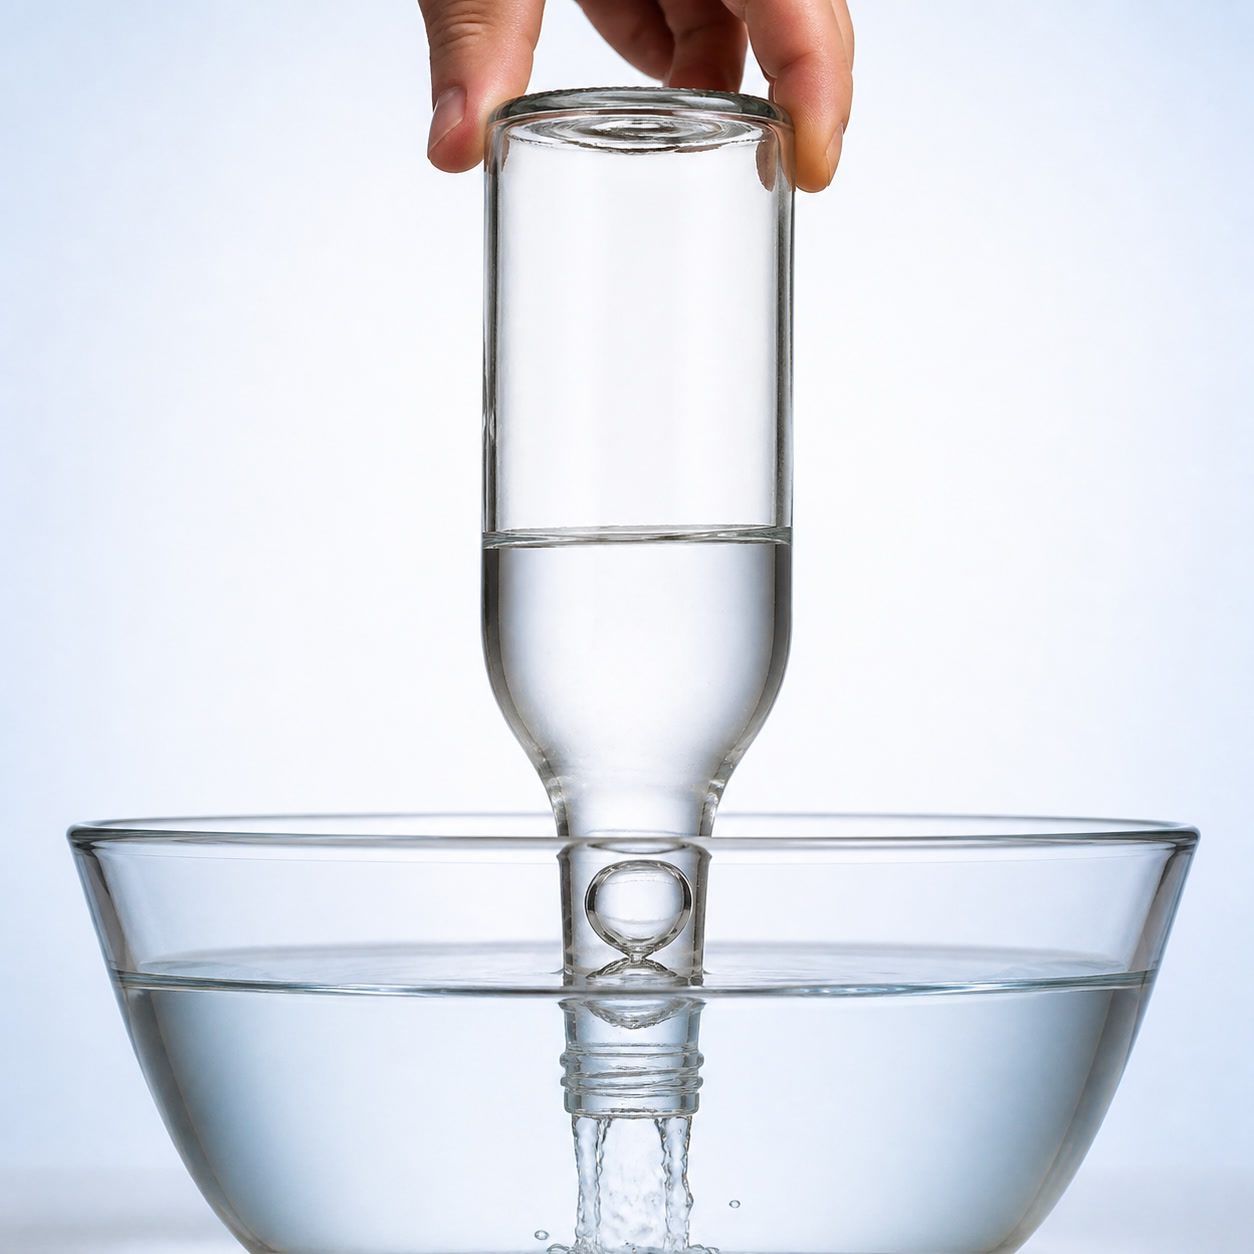
\includegraphics[width=0.42\linewidth]{images/book1/ai/g2-air-glugging-bottle.jpg}

{\small The glugging bottle: as water pours out, big bubbles of \omterm{def:g2:air-around-us:air}{air} fight their way in --- the ``empty'' space must be filled.}
\end{omfigure}

\begin{remark}[No such thing as an empty bottle]\label{rem:g2:air-around-us:noempty}
From now on, be suspicious of the word ``empty''. The empty bottle,
the empty glass, the empty box: all full of \omterm{def:g2:air-around-us:air}{air}, right up to the
brim. Truly empty --- with nothing at all inside, not even \omterm{def:g2:air-around-us:air}{air} ---
is very hard to arrange, and one day you will meet the strange name
scientists give it.
\end{remark}

\section{Air pushes}

\begin{definition}[Wind]\label{def:g2:air-around-us:wind}
\emph{Wind}\index{wind} is \omterm{def:g2:air-around-us:air}{air} on the move. Still \omterm{def:g2:air-around-us:air}{air} brushes
nobody; moving \omterm{def:g2:air-around-us:air}{air} pushes whatever stands in its way --- gently on a
breezy day, hard enough in a storm to bend trees.
\end{definition}

\begin{example}[Air at work]\label{ex:g2:air-around-us:work}
Moving \omterm{def:g2:air-around-us:air}{air} does real jobs: it fills the sails of boats, spins \omterm{def:g2:air-around-us:wind}{wind}
toys, dries the laundry, and carries kites. You make \omterm{def:g2:air-around-us:wind}{wind} yourself
every time you blow out a birthday candle --- your breath is a small
private gust, strong enough to push the flame right off its wick.
\end{example}

\begin{example}[Try it: the balloon jet]\label{ex:g2:air-around-us:balloon}
Blow up a balloon and hold its neck shut. Inside, squeezed \omterm{def:g2:air-around-us:air}{air} is
waiting. Let go: the \omterm{def:g2:air-around-us:air}{air} rushes out backward, and the balloon shoots
forward across the room, wobbling wildly. The escaping \omterm{def:g2:air-around-us:air}{air} pushes
the balloon --- a tiny cousin of the way squeezed-out gas pushes
real rockets.
\end{example}

\begin{omfigure}
\begin{tikzpicture}[scale=0.85]
  % balloon body and its open neck
  \draw[thick, fill=omThm, fill opacity=0.3]
    (4.75,1.3) ellipse (1.4 and 0.95);
  \draw[thick, fill=omThm, fill opacity=0.3]
    (3.44,1.55) .. controls (3.2,1.48) .. (3.02,1.52)
    -- (3.02,1.08) .. controls (3.2,1.12) .. (3.44,1.05) -- cycle;
  % escaping air, fanning backward
  \draw[-Stealth, omDef, thick] (2.85,1.48) -- (1.65,1.66);
  \draw[-Stealth, omDef, thick] (2.85,1.3) -- (1.55,1.3);
  \draw[-Stealth, omDef, thick] (2.85,1.12) -- (1.65,0.94);
  \node[below, font=\small, omDef] at (1.85,0.66) {air rushes out};
  % the flight
  \draw[-Stealth, very thick, omThm] (6.4,1.3) -- (8.1,1.3);
  \node[below right, font=\small, omThm] at (6.3,1.05)
    {the balloon shoots forward};
\end{tikzpicture}

{\small The balloon jet: \omterm{def:g2:air-around-us:air}{air} escaping one way pushes the balloon the
other way.}
\end{omfigure}

\begin{remark}[Air is precious]\label{rem:g2:air-around-us:breathe}
The most important push of all happens quietly in your chest: with
every breath, \omterm{def:g2:air-around-us:air}{air} flows in, your body keeps a little of what it
needs, and the rest flows out. People, cats, birds, even fish (who
sip the \omterm{def:g2:air-around-us:air}{air} hidden in water) all need their share. Invisible does
not mean unimportant --- with \omterm{def:g2:air-around-us:air}{air} it means the opposite.
\end{remark}

\section{Exercises}

\begin{exercise}[$\star$]\label{exo:g2:air-around-us:1}
Name three clues, seen this week, that \omterm{def:g2:air-around-us:air}{air} is real --- without using
any experiment from a book.
\end{exercise}

\begin{exercise}[$\star$]\label{exo:g2:air-around-us:2}
Why does the twisted-shut bag of \cref{ex:g2:air-around-us:catch}
push back when you squeeze it? What is inside?
\end{exercise}

\begin{exercise}[$\star$]\label{exo:g2:air-around-us:3}
In the dry-towel dive, why does the water not reach the towel? Say
it with the chapter's words: what keeps its room?
\end{exercise}

\begin{exercise}[$\star$]\label{exo:g2:air-around-us:4}
What must you \emph{not} do with the glass during the dry-towel
dive, and what would happen to the towel if you did?
\end{exercise}

\begin{exercise}[$\star$]\label{exo:g2:air-around-us:5}
What is the glug-glug of a bottle filling underwater? What goes out,
what comes in, and why must they take turns?
\end{exercise}

\begin{exercise}[$\star$]\label{exo:g2:air-around-us:6}
``Pass me the empty bottle.'' What is really inside an empty
bottle? (See \cref{rem:g2:air-around-us:noempty}.)
\end{exercise}

\begin{exercise}[$\star$]\label{exo:g2:air-around-us:7}
What is \omterm{def:g2:air-around-us:wind}{wind}, in the words of \cref{def:g2:air-around-us:wind}? Give
two jobs that moving \omterm{def:g2:air-around-us:air}{air} does.
\end{exercise}

\begin{exercise}[$\star$]\label{exo:g2:air-around-us:8}
When the balloon jet flies, which way does the \omterm{def:g2:air-around-us:air}{air} rush out, and
which way does the balloon go?
\end{exercise}

\begin{exercise}[$\star\star$]\label{exo:g2:air-around-us:9}
A funnel sits snugly in the neck of a bottle, sealed tight all
around with sticky putty. Ana pours water into the funnel --- and
after a small gulp, the water just sits in the funnel, refusing to
go down into the bottle. Explain what blocks it, and propose the
one-second fix.
\end{exercise}

\begin{exercise}[$\star\star$]\label{exo:g2:air-around-us:10}
Underwater in the bath, tip a glass full of \omterm{def:g2:air-around-us:air}{air} so its mouth faces a
glass full of water, also underwater. Can you pour the \omterm{def:g2:air-around-us:air}{air}
\emph{upward} from one glass into the other? Describe what you would
see, and why the bubbles go up while poured water goes down.
\end{exercise}
